% !TeX spellcheck = it_IT
\documentclass[10pt,a4paper]{article}

\usepackage[utf8]{inputenc}
\usepackage[T1]{fontenc}	
\usepackage[italian]{babel}
\usepackage{amsmath}
\usepackage{amsfonts}
\usepackage{amssymb}
\usepackage{graphicx}

\usepackage[left=2cm,right=2cm,top=2cm,bottom=2cm]{geometry}
\geometry{a4paper}

\usepackage{booktabs} % for much better looking tables
\usepackage{verbatim}
\usepackage{subfig} % make it possible to include more than one captioned figure/table in a single 

\usepackage{fancyhdr} % This should be set AFTER setting up the page geometry
\pagestyle{fancy} % options: empty , plain , fancy
\renewcommand{\headrulewidth}{0pt} % customise the layout...
\lhead{}\chead{}\rhead{}
\lfoot{}\cfoot{\thepage}\rfoot{}

%%% SECTION TITLE APPEARANCE
\usepackage{sectsty}
%\allsectionsfont{\sffamily\mdseries\upshape} % (See the fntguide.pdf for font help)
% (This matches ConTeXt defaults)

% pacchetti che mi fanno schifo ma uso lo stesso (Bob è scemo, ma anche Ale...)
\usepackage[cdot, thickqspace, squaren]{SIunits}
% macro che mi piacciono
\def\code#1{\texttt{#1}}


\title{Esercitazione 6: Amplificatore operazionale\\ \Large{\emph{Circuiti lineari}}}

\author{Gruppo BE \\ Alessandro Candido, Roberto Ribatti}
\date{\today}
\begin{document}
\maketitle

\section{Scopo e strumentazione}
Misurare le caratteristiche di amplificatori invertenti e non invertenti realizzati con un op-amp TL081, da alimentare tra +15 V e -15V.
La strumentazione usata è quella presente sul banco di lavoro, più il suddetto transistor.

\section{Amplificatore invertente}
Si è realizzato l'amplificatore invertente mostrato in \figurename{\ref{circuito_amp_inv}} e si sono scelte le resistenze $R_1$ e $R_2$ rispettivamente di $\unit{10}{k\ohm}$ e $\unit{100}{k\ohm}$ in modo da avere un impedenza di ingresso pari a $R_1$, maggiore di $\unit{1}{k\ohm}$ e un guadagno pari a $R_2/R_1 \sim 10$, come richiesto. Di seguito i valori misurati delle resistenze:

\begin{table}[h!]
	\centering
	\begin{tabular}{cc}
		$R_1 = \unit{9.89 \pm 0.09}{k\ohm}$  & $R_2 = \unit{98.5 \pm 0.9}{k\ohm}$
	\end{tabular}
\end{table}

\subsection{Guadagno e linearità}
Si è misurata quindi la risposta del circuito ad un segnale sinusoidale di frequenza fissata $f = \unit{4.62 \pm 0.05}{k\hertz}$ al variare della tensione picco-picco del segnale in ingresso. I dati raccolti sono elencati in appendice in \tablename{\ref{tab:inv_amp_gain}}.

Dall'analisi del segnale all'oscilloscopio (vedi \figurename{\ref{fig:inv_amp}}) è visibile lo sfasamento di mezzo periodo tra i segnali, come atteso.

\begin{figure}[h!]
	\centering
	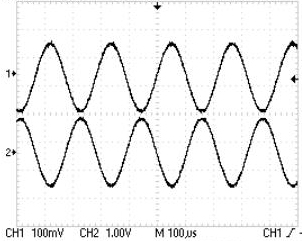
\includegraphics[width=0.5\textwidth]{../oscilloscopio/dinverting.jpg}
	\caption{Inversione di fase nell'amplificatore invertente}
	\label{fig:inv_amp}
\end{figure}

I dati mostrano un chiaro comportamento lineare fino a tensioni in ingresso di $\sim \unit{2.9}{\volt}$ cioè per tensioni di uscita vicine a $\unit{30}{\volt}$, in pratica il regime in cui l'op-amp è lineare. Si è fittato il guadagno nella zona lineare, i risultati e grafici del fit sono riportati di seguito:

\begin{table}[h!]
	\centering
	\begin{tabular}{ccc}
		$|A_v| = 9.72 \pm 0.08$  & intercetta: $\unit{0.04 \pm 0.03}{\volt}$ & $\chi^2/ndof= 8.5 / 23$
	\end{tabular}
\end{table}
Il guadagno misurato è compatibile con quello atteso dalla teoria ($|A_v|^{exp} = 9.96 \pm 0.13$) a meno di $2\sigma$.
\begin{figure}[h!]
	\centering
	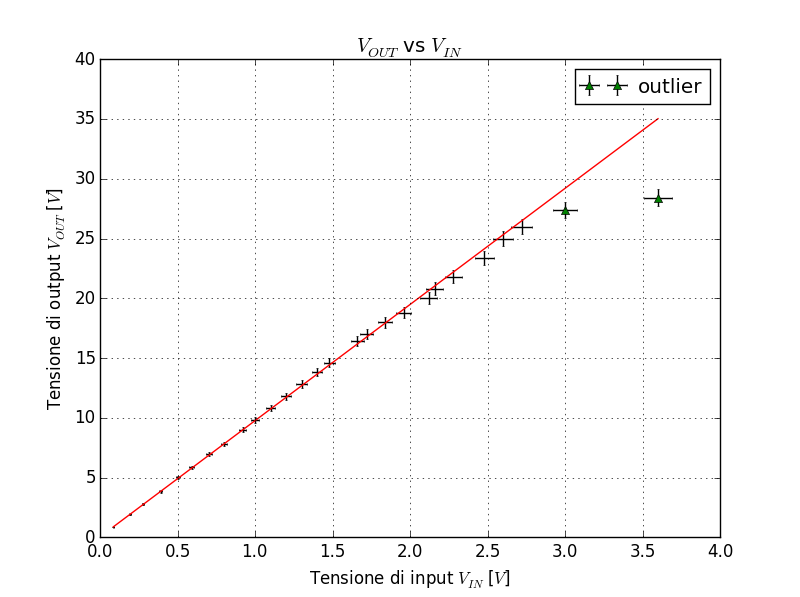
\includegraphics[width=0.85\textwidth]{../grafici/fit_inv_amp_gain.pdf}
	\caption{Guadagno amplificatore invertente}
	\label{fig:inv_amp_gain}
\end{figure}
 
\subsection{Impedenza d'ingresso}
Si è proceduto alla misura della resistenza di ingresso, per farlo si è posta una resistenza $R* = \unit{9.96 \pm 0.09}{k\ohm}$ in serie all'ingresso del circuito e si è misurata la caduta di potenziale ai capi della stesso ottenendo:

\begin{table}[h!]
	\centering
	\begin{tabular}{cc}
		$V_1 = \unit{2.88 \pm 0.10}{\volt}$  &  $V_2\unit{1.44 \pm 0.05}{\volt}$
	\end{tabular}
\end{table}

L'impedenza di ingresso misurata è quindi $R_{IN}=\unit{10.0 \pm 1.0}{k\ohm}$, ampiamente compatibile con quella attesa pari a $R_1$.

\subsection{Risposta in frequenza}
Si è studiata quindi la risposta in frequenza del circuito, per una tensione picco-picco in ingresso pari a $V = \unit{496 \pm 12}{\milli\volt}$. I dati acquisiti sono riportati in appendice in \tablename{\ref{tab:inv_amp_f_domain}}.

Dal grafico in \figurename{\ref{palle}} è chiaro che il guadagno è costante fino ad un frequenza di $\sim \unit{200}{k\hertz}$, da questo punto in poi il guadagno sembra calare linearmente con un tasso di $\sim \unit{20}{\deci\bel /decade}$ per un primo tratto fino a $f \sim {600}{k\hertz}$, per frequenze superiori la pendenza sembra aumentare.

Si è provato a fittare questo comportamento (il grafico del fit è riportato in \figurename{\ref{rette}}), le pendenze fittate sono state $p_1 = \unit{-20.1 \pm 1.8}{\deci\bel/decade}$ per il primo tratto e $p_2 =\unit{-33.3 \pm 1.2}{\deci\bel/decade}$ per il secondo tratto.

\begin{figure}[h!]
	\centering
	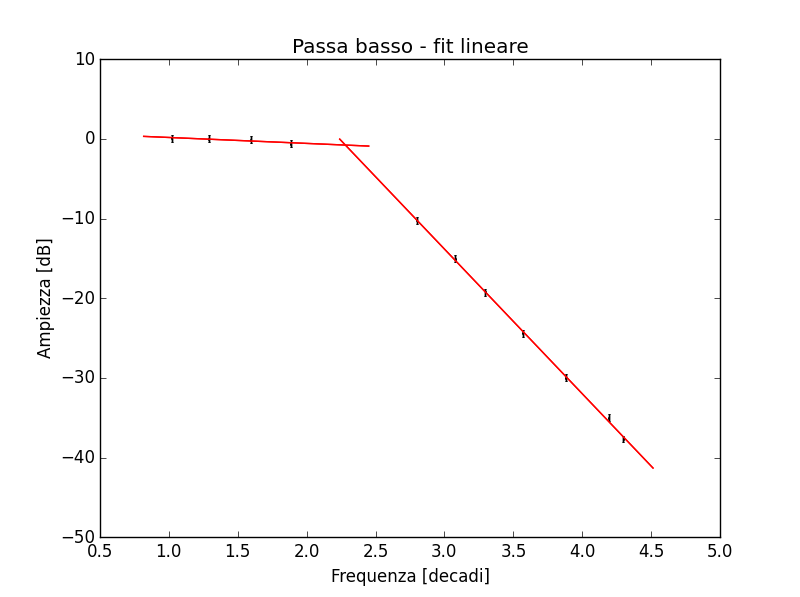
\includegraphics[width=0.8\textwidth]{../grafici/fit_rette.pdf}
	\caption{fit del guadagno per alte frequenze}
	\label{rette}
\end{figure}

Si è deciso quindi di fittare la risposta in frequenza dell'amplificatore invertente con il modello di un filtro passa basso escludendo i dati presi a frequenze sopra $\sim \unit{600}{k\hertz}$ che come visto prima non rispettano la legge di decrescita attesa.  Si riportano di seguito i risultati del fit e il grafico.

\begin{table}[h!]
	\centering
	\begin{tabular}{ccc}
	$|A_v| = 10.15 \pm 0.13$	&	$f_0 = \unit{214 \pm 6}{k\hertz}$	&	$\chi^2/ndof = 23 / 20$\\
	\end{tabular}
\end{table}

\begin{figure}[h!]
	\centering
	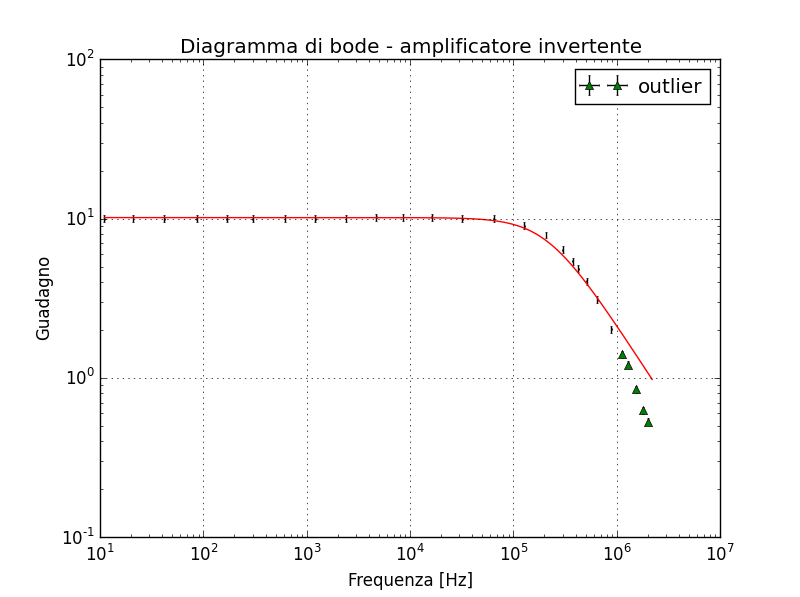
\includegraphics[width=0.8\textwidth]{../grafici/fit_inv_amp_f_domain.pdf}
	\caption{Grafico dei dati e del fit}
	\label{palle}
\end{figure}

Il guadagno di centro banda fittato è compatibile con quello atteso dalla teoria e con quello misurato al punto precedente.
L'andamento ad alte frequenze è probabilmente influenzato dallo slew rate che in questo range distorce significativamente il segnale.
\pagebreak
\subsection{Slew rate}
Si è misurato lo slew rate dell'op-amp inviando in ingresso un'onda quadra di frequenza $\unit{1000 \pm 10}{\hertz}$, ottenendo una discesa pari a  $\Delta V = \unit{9.44 \pm 0.24}{\volt}$ in un tempo $\Delta t = \unit{740 \pm 7}{\nano\second}$.

Lo slew rate misurato è quindi pari a $\unit{12.8 \pm 0.3}{\volt/\micro\second}$, mentre il datasheet riporta un valore tipico di $\unit{13}{\volt/\micro\second}$.

%gli errori sulle frequenze li abbiamo messi sempre all'1%?

\section{Amplificatore non invertente}

Si è montato l'amplificatore non invertente in \figurename{\ref{circuito_non_inv}} con i seguenti valori dei componenti:

\begin{table}[h!]
	\centering
	\begin{tabular}{cc}
		$R_1 = \unit{218 \pm 3}{\ohm}$  & $P_1 = \unit{100}{k\ohm}$
	\end{tabular}
\end{table}

Si sono misurati al variare della posizione del potenziometro il guadagno (misurato a basse frequenze $f < \unit{100}{\hertz}$, dove sicuramente l'amplificatore è in regime lineare) e la frequenza di taglio superiore. I dati acquisiti sono riportati in appendice in \tablename{\ref{tab:gain_bandwidth}}. Per verificare che il prodotto banda-guadagno rimanesse costante si è fittato con una retta il guadagno (in decibel) in funzione del logaritmo della frequenza. I risultati e i grafici del fit sono riportati di seguito (a è il coefficiente angolare e b l'intercetta):

\begin{table}[h!]
	\centering
	\begin{tabular}{ccc}
		$a = \unit{-20.49 \pm 0.18}{\deci\bel /decade}$  &  $b = \unit{128.8 \pm 0.8}{\deci\bel}$ & $\chi^2/ndof= 14.8 / 13$
	\end{tabular}
\end{table}

\begin{figure}[h!]
	\centering
	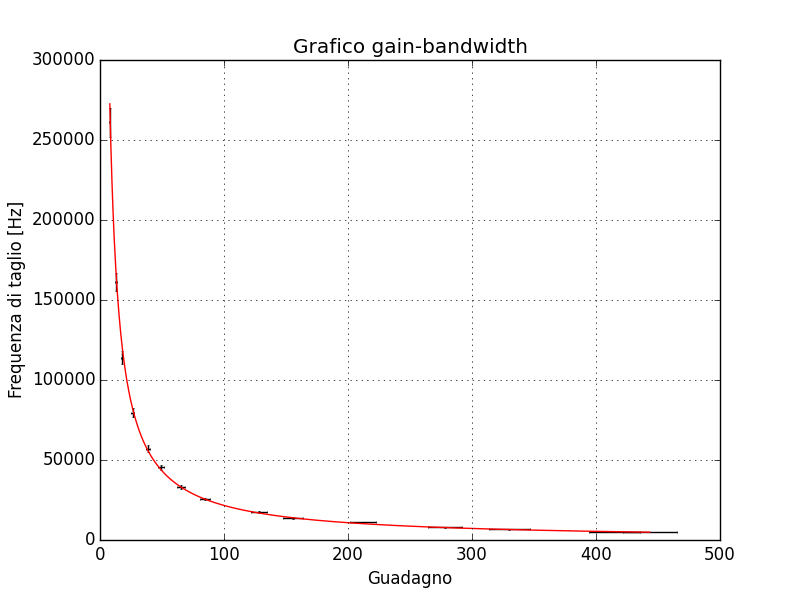
\includegraphics[width=0.8\textwidth]{../grafici/fit_gain_bandwidth.pdf}
	\caption{Grafico e fit banda-guadagno}
\end{figure}

Il prodotto banda guadagno, ovvero l'intersezione della retta fittata con l'asse a $\unit{0}{\deci\bel}$ varrà perciò\footnote{propagando l'errore tenendo conto della covarianza}: $Af_h=\unit{1.93\pm0.12}{\mega\hertz}$, che è compatibile con il grafico presente nel datasheet riportato in \figurename{\ref{fig:open_loop_stocazzo}}.

\begin{figure}[h!]
	\centering
	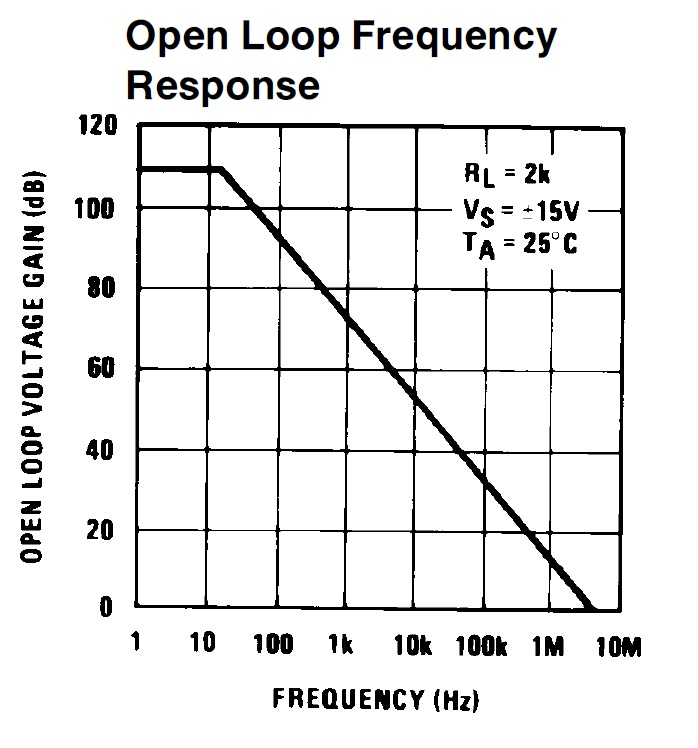
\includegraphics[width=0.4\textwidth]{../grafici/open_loop_frequency.jpg}
	\caption{Grafico guadagno-banda dal datasheet}
	\label{fig:open_loop_stocazzo}
\end{figure}

\section{Circuito integratore}

I valori dei componenti utilizzati nel montaggio del circuito sono:

\begin{table}[h!]
\centering
\begin{tabular}{ccc}
$R_1 = \unit{984 \pm 9}{ohm}$	&	$R_2 = \unit{9.95 \pm 0.09}{\kilo\ohm}$	&	$C = \unit{45.4 \pm 1.8}{\nano\farad}$
\end{tabular}
\end{table}

\subsection{Risposta in frequenza}
Si è misurata la risposta del circuito a un ingresso sinusoidale a varie frequenze. Si riportano i dati relativi in appendice in \tablename{\ref{tab:lowpass}}, e i grafici di seguito in \figurename{\ref{fig:lowamp}} e \figurename{\ref{fig:lowph}}.

\begin{figure}[h!]
\centering
	\begin{minipage}[h!]{0.48\textwidth}
		\centering
		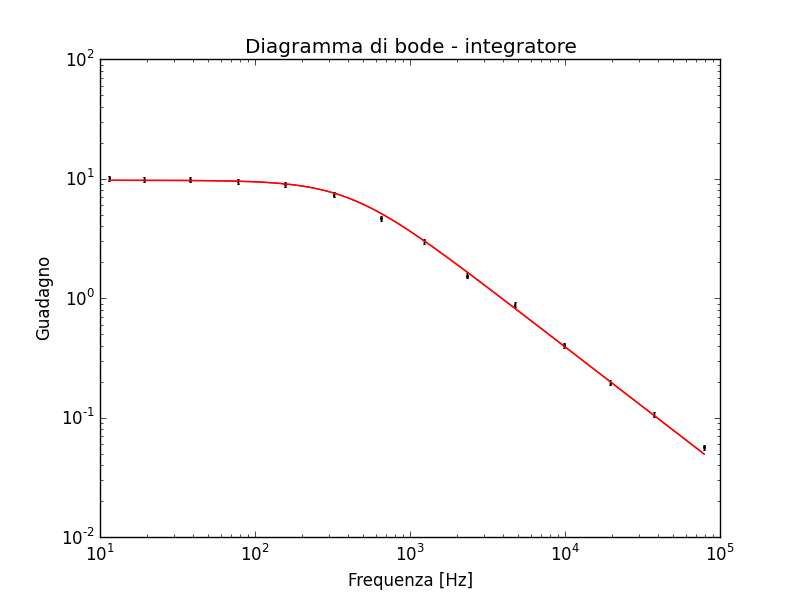
\includegraphics[width=\textwidth]{../grafici/fit_module_low_pass.pdf}
		\caption{Grafico del fit }
		\label{fig:lowamp}
	\end{minipage}
	\begin{minipage}[h!]{0.48\textwidth}
		\centering
		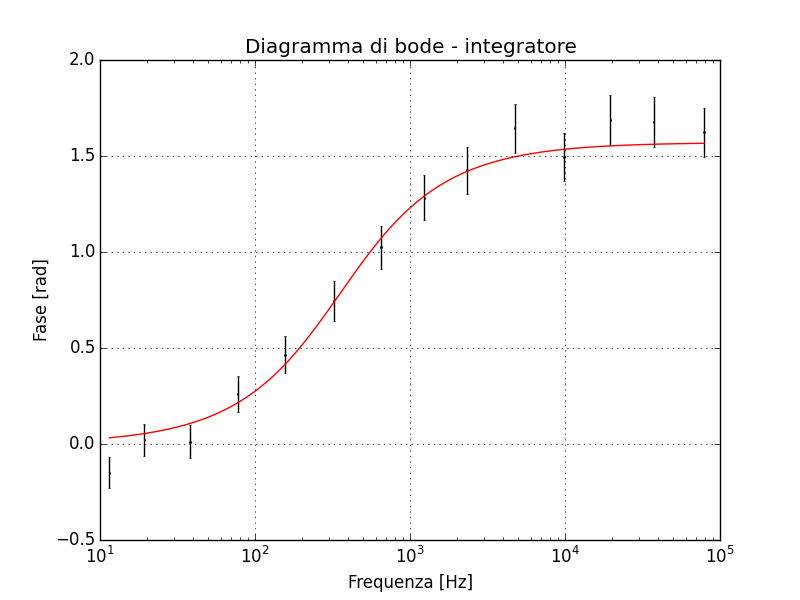
\includegraphics[width=\textwidth]{../grafici/fit_phase_low_pass.pdf}
		\caption{Grafico del fit }
		\label{fig:lowph}
	\end{minipage}
\end{figure}

Si riportano nella tabella di seguito i risultati del fit:

\begin{table}[h!]
\centering
\begin{tabular}{c|ccc}
amplitude	&	$A_0 = 9.71 \pm 0.22$	&	$f_0 = \unit{404 \pm 12}{\hertz}$	&	$\chi^2/ndof = 15.6 / 12$\\
phase		& &	$f_0 = \unit{350 \pm 40}{\hertz}$	&	$\chi^2/ndof = 10.7 / 13$
\end{tabular}
\end{table}

\noindent Dove si sono usati i seguenti simboli:
\begin{itemize}
\item $A_0$ è il guadagno di centro banda, in questo caso è il guadagno a basse frequenze;
%\item $\varphi_0$ è lo sfasamento per frequenze prossime allo 0;
\item $f_0$ è la frequenza di taglio dell'integratore.
\end{itemize}

Si nota dunque che le due misure della frequenza di taglio sono compatibili, a meno di $\sim 1\sigma$.

\subsection{Risposta all'onda quadra}

Qualitativamente il comportamento osservato per la risposta del circuito all'onda quadra è esattamente quello di un integratore, almeno a $\unit{10}{\kilo\hertz}$, come si osserva dalla \figurename{\ref{fig:intsq}}.

\begin{figure}[h!]
	\begin{minipage}[t]{0.45\textwidth}
		\centering
		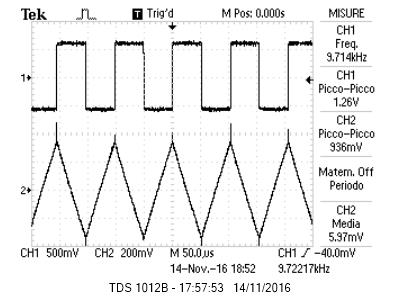
\includegraphics[width=1\textwidth]{../oscilloscopio/sqint.jpg}
	\end{minipage}
	\begin{minipage}[t]{0.45\textwidth}
		\centering
		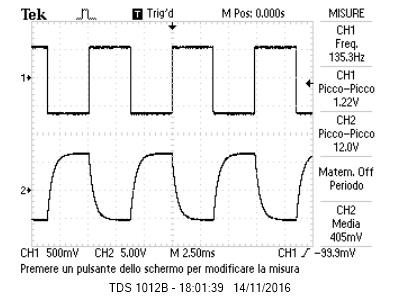
\includegraphics[width=1\textwidth]{../oscilloscopio/sqexp.jpg}
	\end{minipage}
	\caption{Risposta del circuito integratore a un'onda quadra in ingresso}
	\label{fig:intsq}
\end{figure}

Cambiando la frequenza del segnale di input si osserva che per frequenze maggiori il segnale viene ulteriormente attenuato, ma qualitativamente preserva il funzionamento come derivatore, mentre per frequenze più basse il condensatore ha il tempo di caricarsi e si può osservare una serie di esponenziali dovuti proprio a queste cariche e scariche, sempre in \figurename{\ref{fig:intsq}}.

% c'è da dire cosa ci si aspetta per l'ampiezza dell'onda in uscita:
% - slew rate * tempo a disposizione (semiperiodo)
% - carica del condensatore(con il tau del passa basso)
% mi serve il valore dello slew rate misurato ai punti precedenti

\subsection{Confronto con i risultati attesi}

Il valore della frequenza di taglio attesa è pari a $f_0 = \unit{352 \pm 11}{\hertz}$ ed è compatibile con quella misurata con il fit degli sfasamenti, ma anche con quanto ottenuto dal fit dei guadagni, a meno di $2\sigma$.

Come risulta dai grafici mostrati in \figurename{\ref{fig:lowamp}} e  \figurename{\ref{fig:lowph}} il comportamento del circuito in esame è lo stesso di un passa-basso, con una funzione di trasferimento moltiplicata per un fattore $-R_2/R_1$, che quindi aumenta il guadagno massimo e inverte l'output, aggiungendo un $\pi$ alla fase di quest'ultimo.

La resistenza $R_2$ serve a spostare il polo dallo 0, e di conseguenza limitare il guadagno massimo del circuito, che altrimenti andrebbe a coincidere con quello dell'operazionale, un valore non stabilmente fissato. Invece in questo modo il massimo valore del guadagno è pari proprio a  $R_2/R_1$, come scritto sopra.
Idealmente è proprio per questo motivo che compare una frequenza di taglio: se l'amplificatore avesse un guadagno infinito il guadagno del circuito sarebbe una retta in assenza di $R_2$, per cui si comporerebbe da integratore a qualunque frequenza.

\section{Circuito derivatore}

I valori dei componenti usati nel montaggio del circuito coincidono con quelli al punto precedente, cioè quelli usati nel circuito integratore.

\subsection{Risposta in frequenza}

Come nel caso precedente si riportano i dati in appendice in \tablename{\ref{tab:highpass}} e i grafici di seguito, in \figurename{\ref{fig:highamp}} e \figurename{\ref{fig:highph}}.

\begin{figure}[h!]
\centering
	\begin{minipage}[h!]{0.48\textwidth}
		\centering
		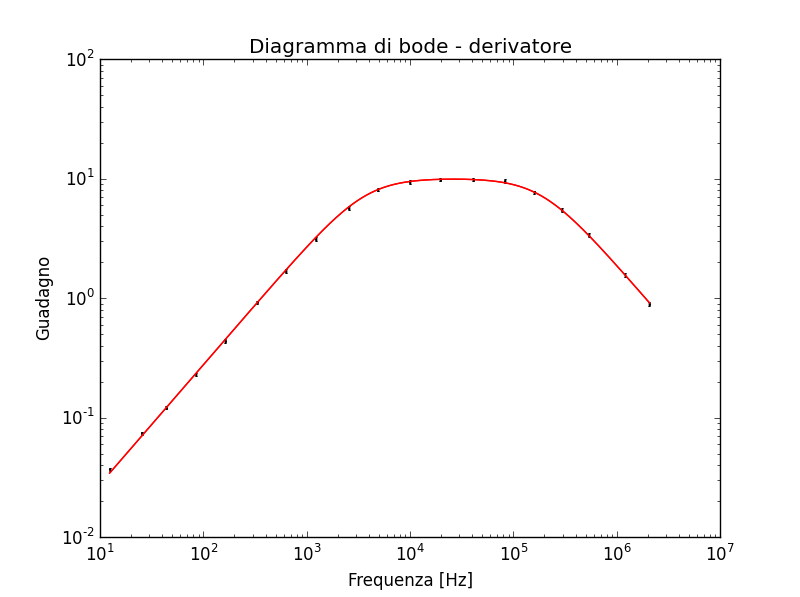
\includegraphics[width=\textwidth]{../grafici/fit_module_high_pass.pdf}
		\caption{Grafico del fit }
		\label{fig:highamp}
	\end{minipage}
	\begin{minipage}[h!]{0.48\textwidth}
		\centering
		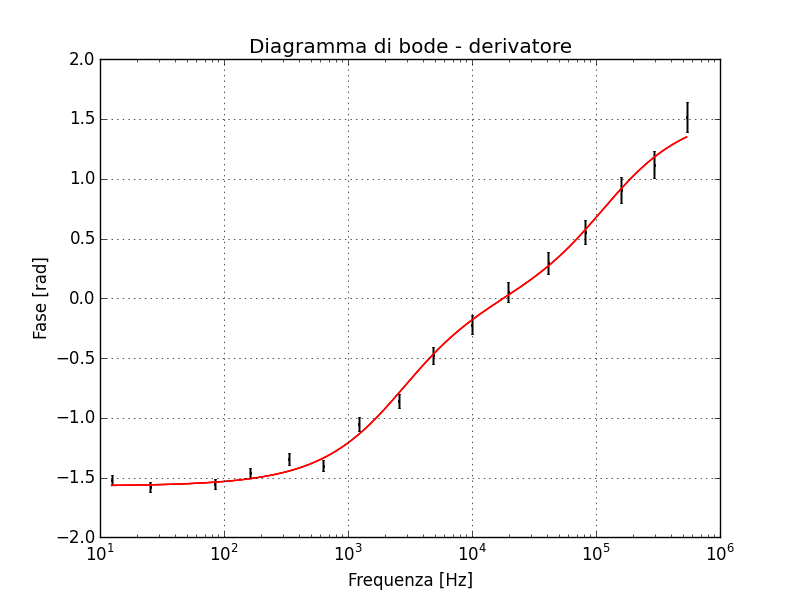
\includegraphics[width=\textwidth]{../grafici/fit_phase_high_pass.pdf}
		\caption{Grafico del fit }
		\label{fig:highph}
	\end{minipage}
\end{figure}

Si riportano nella tabella di seguito i risultati del fit:

\begin{table}[h!]
\centering
\begin{tabular}{c|cccc}
amplitude	&	$A_0 = 10.11 \pm 0.18$	&	$f_1 = \unit{3.64 \pm 0.08}{\kilo\hertz}$	&	$f_2 = \unit{189 \pm 6}{\kilo\hertz}$	&	$\chi^2/ndof = 8.6 / 16$\\
phase		& &	$f_1 = \unit{2.72 \pm 0.2}{\kilo\hertz}$	&	$f_2 = \unit{118 \pm 14}{\kilo\hertz}$	&	$\chi^2/ndof = 14.5 / 14$
\end{tabular}
\end{table}

\noindent Dove si è indicato con $f_1, f_2$ le due frequenze di taglio del circuito. La prima frequenza è relativa al derivatore, cioè quella fissata dal dimensionamento del circuito, mentre la seconda frequenza è quella relativa al taglio delle alte frequenze dovuto 

\subsection{Risposta all'onda triangolare}
Il circuito si comporta come un derivatore alla frequenza di $\sim \unit{100}{\hertz}$, come risulta dall'immagine riportata in \figurename{\ref{fig:trdev}}.

\begin{figure}[h!]
	\centering
	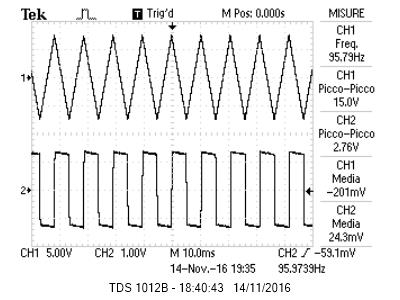
\includegraphics[width=0.5\textwidth]{../oscilloscopio/trdev.jpg}
	\caption{Risposta del circuito derivatore a un'onda triangolare in ingresso}
	\label{fig:trdev}
\end{figure}

Variando la frequenza si ha che per frequenze molto basse il condensatore si carica in un tempo breve rispetto alla durata del periodo, per cui la risposta approssima sempre meglio un'onda quadra, mentre per frequenze troppo elevati il segnale viene mediato, e dunque nuovamente attenuato, come risulta dal grafico in \figurename{\ref{fig:highamp}}.

\subsection{Confronto con i risultati attesi}

Il valore atteso della frequenza di taglio è $f_1 = \unit{3.56 \pm 0.11}{\kilo\hertz}$, ed è perciò compatibile con quella ottenuta dal fit dei guadagni.

La funzione della resistenza $R_1$ è quella di aggiungere un polo, in modo tale da stabilizzare il circuito alle alte frequenze, cioé fissare il valore del massimo guadagno a un valore di progetto determinato dal dimensionamento delle resistenze e del condensatore.

Inoltre il circuito presenta un'altra frequenza di taglio, come si è notato ai punti precedenti. Questa non è prevista da un comportamento ideale del circuito in esame ()in cui l'operazionale abbia una resistenza di ingresso infinita e una di uscita nulla), ma tenendo di conto il comportamento reale dell'operazionale anche la seconda frequenza di taglio è spiegata. Il motivo è il condensatore presente nell'operazionale, lo stesso che porta a uno slew rate finito.

Anche in questo caso il guadagno massimo del circuito è moltiplicato per un valore $-R_2/R_1$, ma stavolta è ottenuto per alte frequenze, o meglio in una certa banda, prima che il segnale venga di nuovo attenuato.

\pagebreak
\section{Appendice: Dati}
Si riportano qui le tabelle di dati usati per i fit e i grafici.

\centering
\begin{figure}[h!]
	\begin{minipage}[c]{0.33\textwidth}
		\resizebox{1\textwidth}{!}{
		\input{../tabelle/tab_inv_amp_gain.txt}}
		\captionof{table}{Guadagnio amplificatore invertente}
		\label{tab:inv_amp_gain}
	\end{minipage}
	\begin{minipage}[c]{0.33\textwidth}
		\resizebox{1\textwidth}{!}{
		\input{../tabelle/tab_inv_amp_f_domain.txt}}
		\captionof{table}{Risposta in frequenza amplificatore invertente}
		\label{tab:inv_amp_f_domain}
	\end{minipage}
	\begin{minipage}[c]{0.33\textwidth}
		\resizebox{1\textwidth}{!}{
			\input{../tabelle/tab_gain_bandwidth.txt}}
		\captionof{table}{Banda/Guadagno}
		\label{tab:gain_bandwidth}
	\end{minipage}
\end{figure}

\begin{figure}[h!]
	\centering
	\resizebox{0.7\textwidth}{!}{
	\input{../tabelle/tab_low_pass.txt}}
	\captionof{table}{Dati relativi al circuito integratore}
	\label{tab:lowpass}
\end{figure}

\begin{figure}[h!]
	\centering
	\resizebox{0.7\textwidth}{!}{
	\input{../tabelle/tab_high_pass.txt}}
	\captionof{table}{Dati relativi al circuito derivatore}
	\label{tab:highpass}
\end{figure}



\end{document}
